\documentclass[letter,11pt]{article}

\usepackage[spanish,es-nodecimaldot]{babel}
\usepackage[utf8]{inputenc}

\usepackage{lmodern}
\usepackage[T1]{fontenc}
\usepackage{textcomp}

\usepackage{framed}
\usepackage[svgnames]{xcolor}
\colorlet{shadecolor}{Gainsboro!50}

\usepackage[labelfont=bf]{caption}
\usepackage{graphicx}
\usepackage{pstricks}

\usepackage{anysize}
\marginsize{3cm}{2cm}{2cm}{3cm}

\usepackage{siunitx}
\usepackage{amsmath}
\usepackage{array}
\usepackage{csquotes}

\usepackage{fancyhdr}
\usepackage{lastpage}
\pagestyle{fancy}
\fancyhf{}
\fancyhead[LE,RO]{Laboratorio de Circuitos Eléctricos I}
\fancyfoot[CO,CE]{\thepage\ de \pageref{LastPage}}

\special{papersize=215.9mm,279.4mm}

\usepackage[
    pdfauthor={Carlos Eduardo Caballero Burgoa},%
    pdftitle={Laboratorio de Circuitos Eléctricos I},%
    pdfsubject={Teorema de Thévenin},%
    colorlinks,%
    citecolor=black,%
    filecolor=black,%
    linkcolor=black,%
    urlcolor=black,
    breaklinks]{hyperref}
\usepackage{breakurl}

\newcommand{\blankpage}{
\newpage
\thispagestyle{empty}
\mbox{}
\newpage
}

\renewcommand{\arraystretch}{1.2}

\begin{document}

\begin{titlepage}
    \begin{center}
        {\Large UNIVERSIDAD MAYOR DE SAN SIMÓN}\\
        \vspace*{0.15cm}
        {\large FACULTAD DE CIENCIAS Y TECNOLOGÍA}\\
        \vspace*{0.10cm}
        DEPARTAMENTO DE ELÉCTRICA-ELECTRÓNICA\\
        \vspace*{3.0cm}
        {\Large \textbf{LABORATORIO DE CIRCUITOS ELÉCTRICOS I}}\\
        \vspace*{0.3cm}
        {\Large \textbf{INFORME No. 4}}\\
        \vspace*{3.5cm}
        {\Large \textbf{TEOREMA DE \emph{THÉVENIN}}}\\
    \end{center}

    \vspace*{6.4cm}
    \leftskip=7.95cm
    \noindent
    \textbf{Estudiante:}\\
    Caballero Burgoa, Carlos Eduardo.\\
    \newline
    \textbf{Carrera:}\\
    Ing. Electromecánica.\\
    \newline
    \textbf{Docente:}\\
    Ing. Marco Antonio Vallejo Camacho.\\
    \newline
    \textbf{Grupo:} 3E.\\
    \textbf{Fecha de entrega:} 14 de Mayo del 2024.\\
\end{titlepage}

\section{Cálculos previos}

\begin{figure}[!h]
\centering
\includegraphics[scale=0.168]{resources/preinforme1.eps}
\end{figure}

\begin{figure}[!h]
\centering
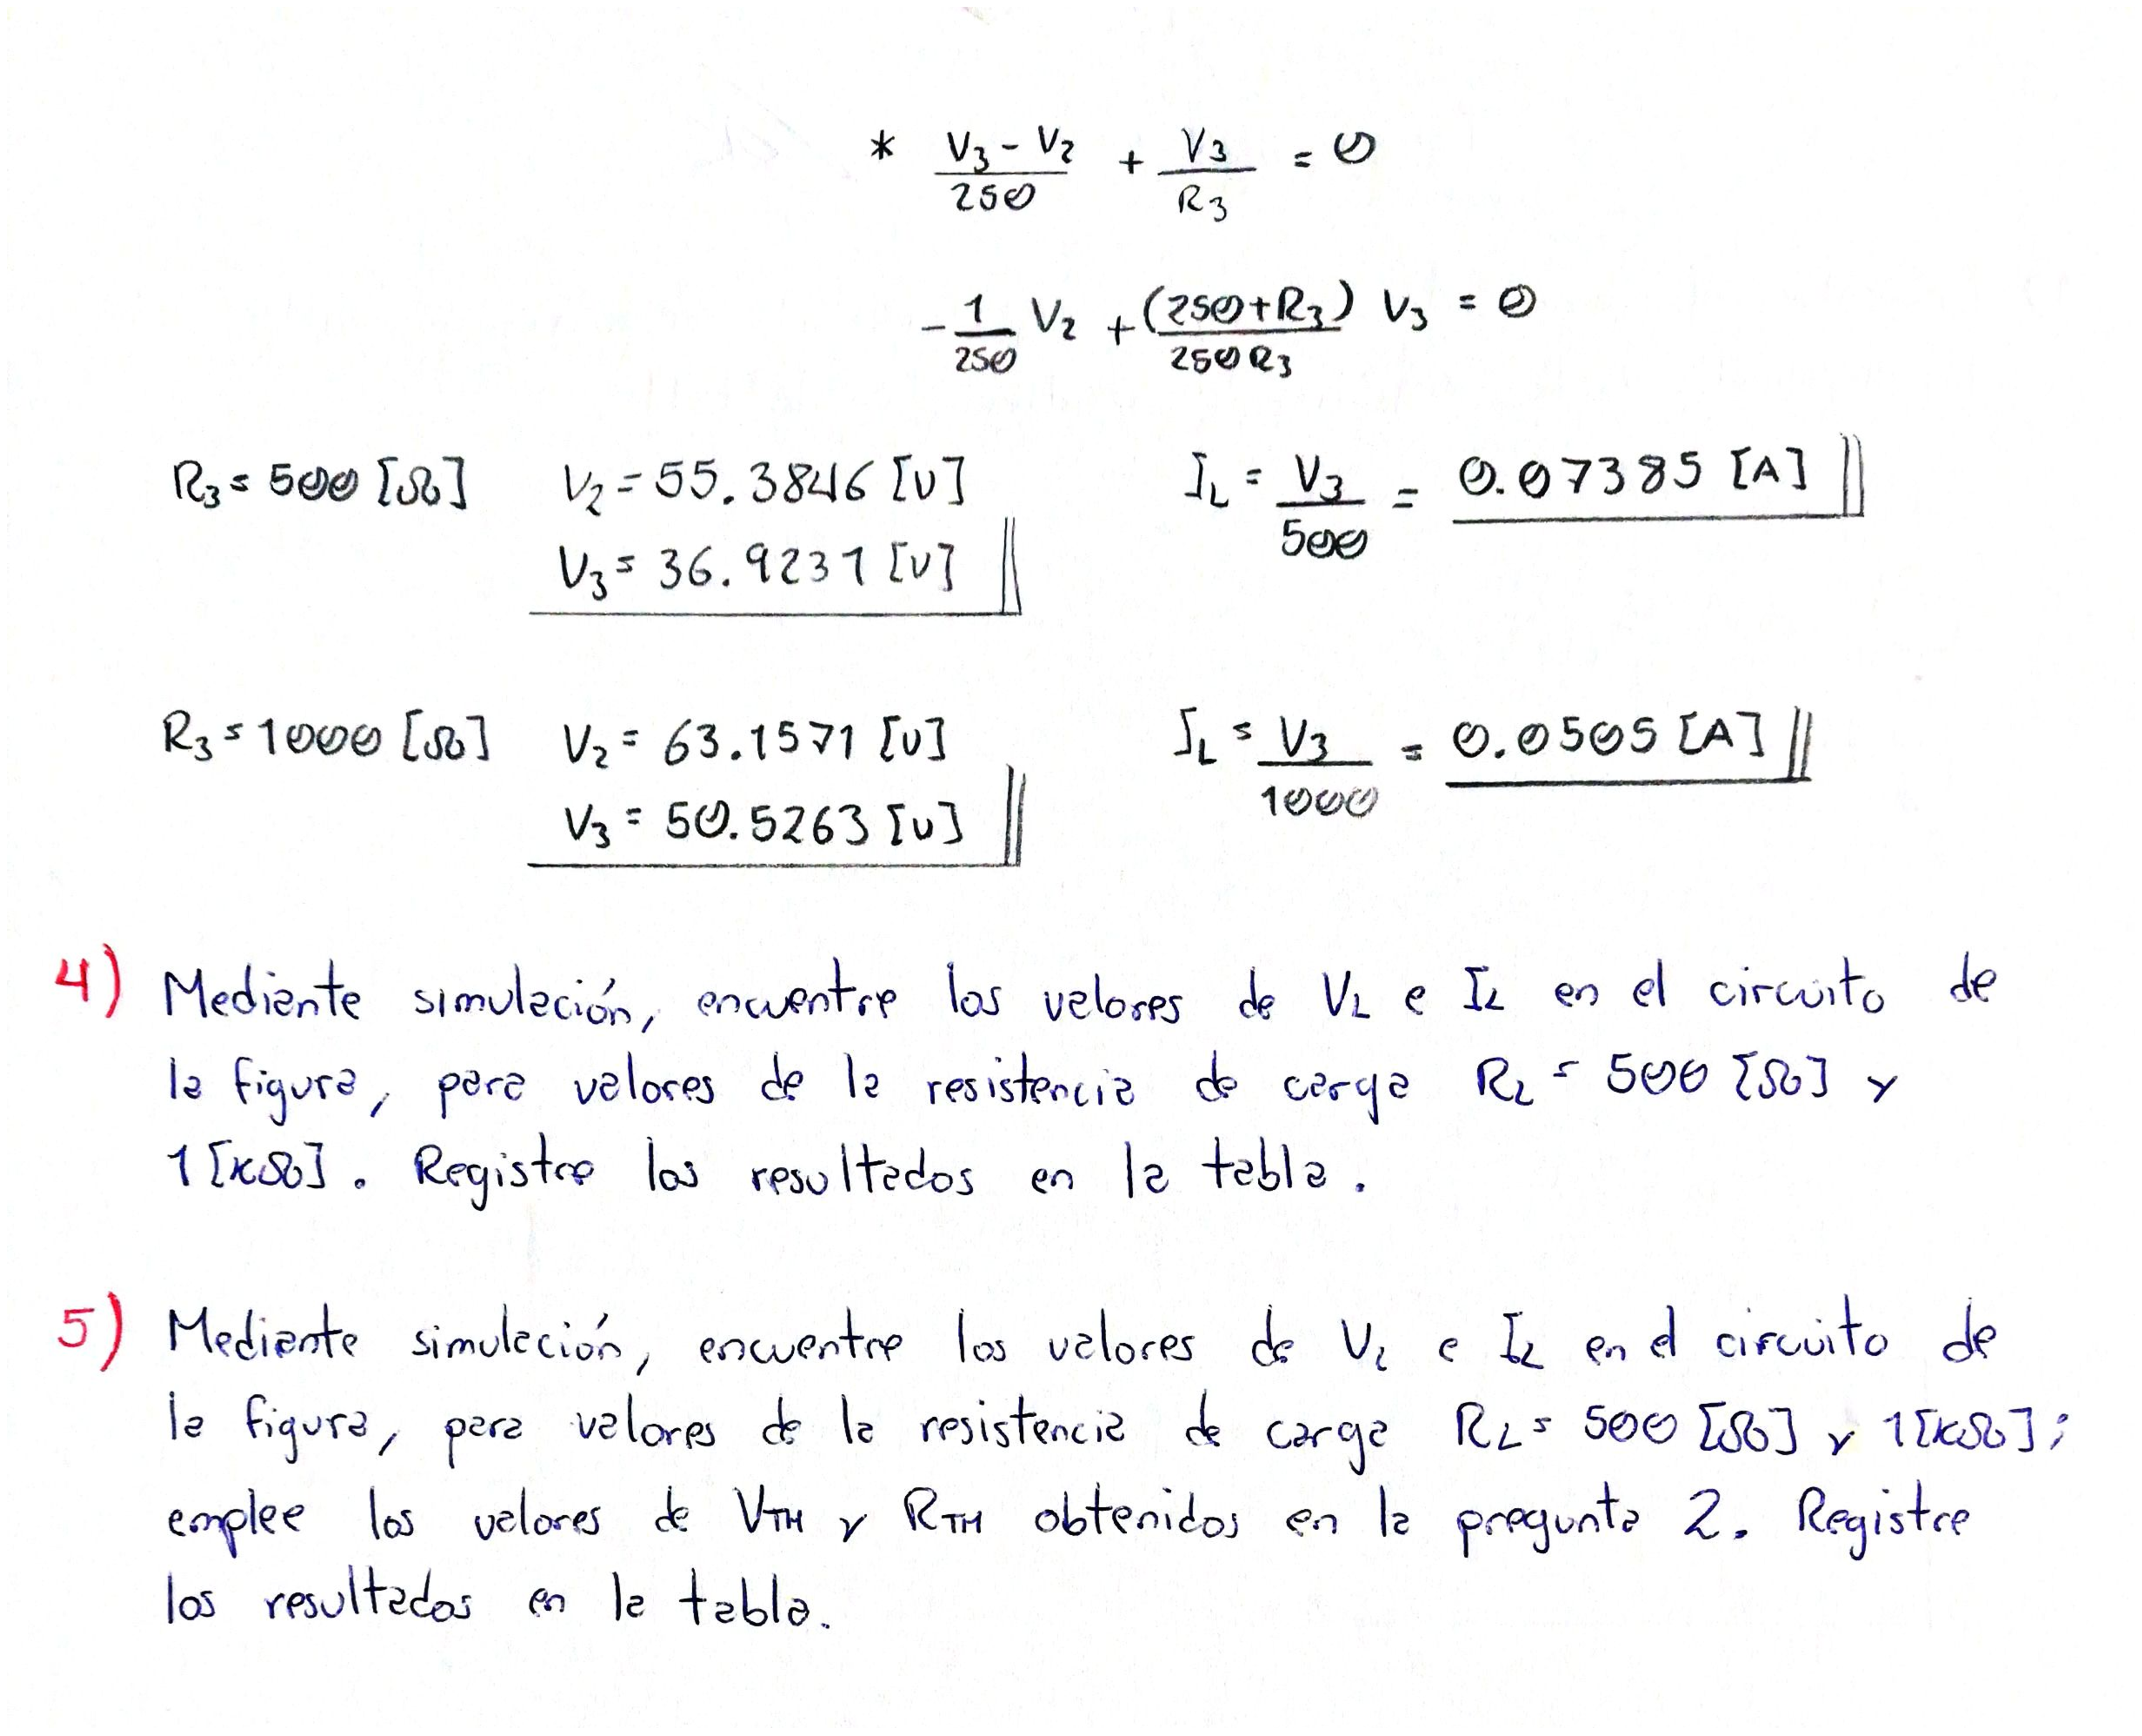
\includegraphics[scale=0.168]{resources/preinforme2.eps}
\end{figure}

\section{Simulación}
Se utilizó el software \emph{Quite Universal Circuit Simulator.} para simular
los circuitos, estos pueden verse en la figura (\ref{simulacion1}),
(\ref{simulacion2}) y (\ref{simulacion3}).

\begin{figure}[!h]
\centering
\includegraphics[scale=0.52]{simulation/practica4.1.eps}
\caption{Simulación para el calculo del equivalente de \emph{Thévenin}.}
\label{simulacion1}
\end{figure}

\begin{figure}[!h]
\centering
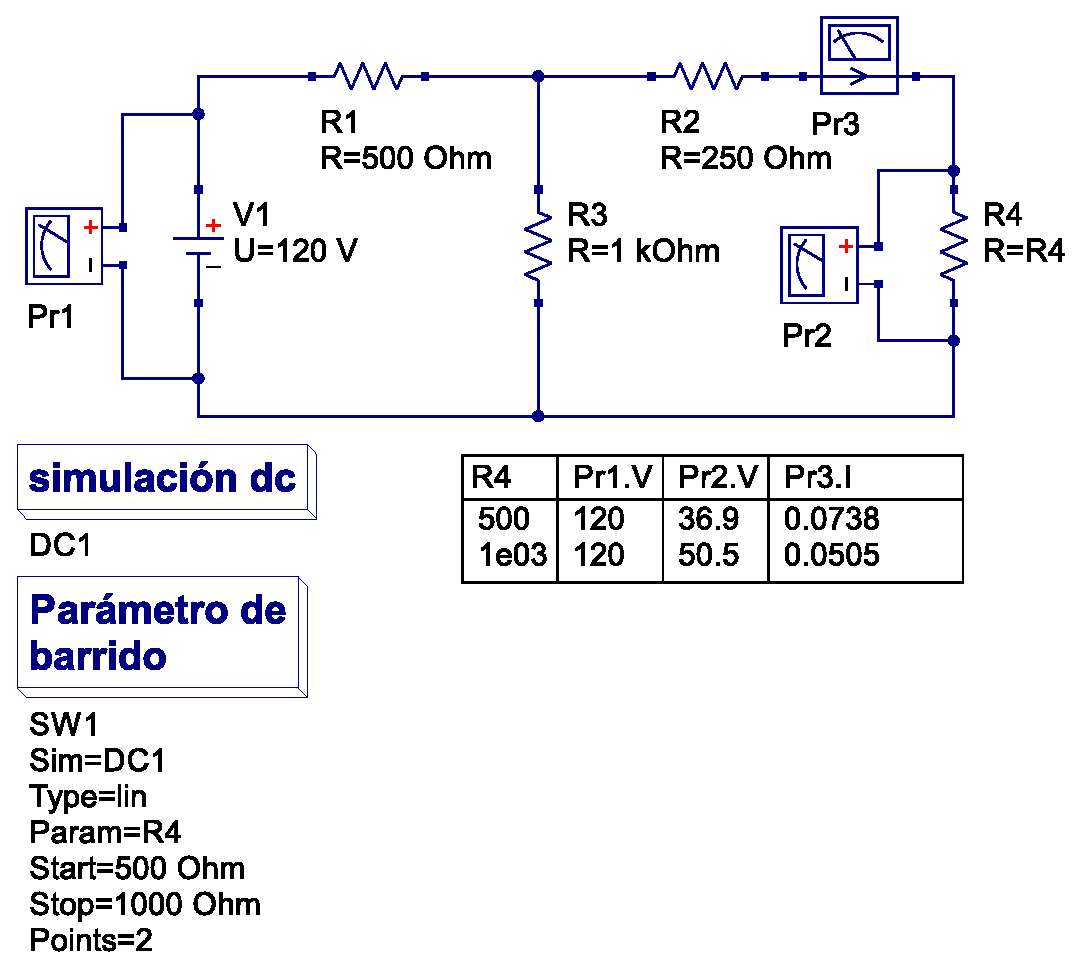
\includegraphics[scale=0.60]{simulation/practica4.2.eps}
\caption{Simulación del circuito de practica.}
\label{simulacion2}
\end{figure}

\begin{figure}[!h]
\centering
\includegraphics[scale=0.64]{simulation/practica4.3.eps}
\caption{Simulación del circuito con el equivalente de \emph{Thévenin}.}
\label{simulacion3}
\end{figure}

\section{Tablas y mediciones}
En la figura (\ref{tablas}), se adjunta la hoja de resultados provista en la
guía de laboratorio, rellenada con la información teórica, simulada y las
mediciones realizadas en laboratorio.

\begin{figure}[!h]
\centering
\includegraphics[scale=0.18]{resources/preinforme3.eps}
\caption{Tabla de resultados.}
\label{tablas}
\end{figure}

\section{Cuestionario}

\begin{enumerate}

\item \textbf{A partir del equivalente \emph{Thévenin} obtenido en el
laboratorio y utilizando la transformación de fuentes, encuentre el equivalente
de \emph{Norton}.} \\

\begin{figure}[!h]
\centering
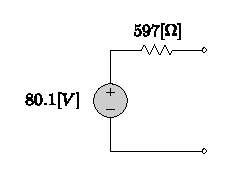
\includegraphics[width=0.23\textwidth]{resources/figura1.eps}
\end{figure}

\begin{equation*}
    I_{N} = \frac{V_{TH}}{R_{TH}}
          = \frac{80.1 [V]}{597 [\Omega]}
          = 0.13 [A]
\end{equation*}

\begin{figure}[!h]
\centering
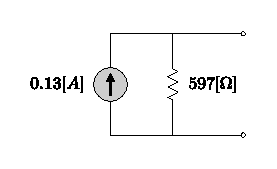
\includegraphics[width=0.27\textwidth]{resources/figura2.eps}
\end{figure}

\item \textbf{Determine el equivalente \emph{Thévenin} viste desde las
terminales $A-B$ del circuito mostrado en la figura a continuación. Trabaje con
la fuente $V_0$ y su resistencia interna $R_0$ en forma literal.}\\

\begin{figure}[!h]
\centering
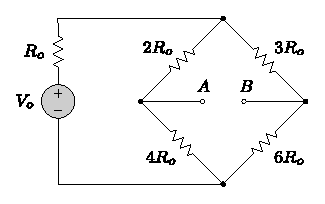
\includegraphics[width=0.30\textwidth]{resources/figura3.eps}
\end{figure}

Calculando la resistencia de \emph{Thévenin}:

\begin{figure}[!h]
\centering
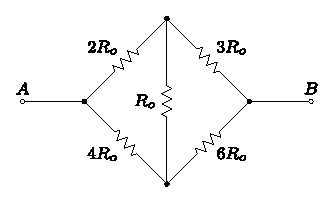
\includegraphics[width=0.30\textwidth]{resources/figura4.eps}
\end{figure}

Aplicando una transformación delta-estrella:

\begin{equation*}
    R_1 = \frac{2R_o\,4R_o}{2R_o+4R_o+R_o} = \frac{8}{7}R_o
\end{equation*}
\begin{equation*}
    R_2 = \frac{2R_o\,1R_o}{2R_o+4R_o+R_o} = \frac{2}{7}R_o
\end{equation*}
\begin{equation*}
    R_3 = \frac{4R_o\,1R_o}{2R_o+4R_o+R_o} = \frac{4}{7}R_o
\end{equation*}

\begin{figure}[!h]
\centering
\includegraphics[width=0.40\textwidth]{resources/figura5.eps}
\end{figure}

\begin{equation*}
    R_4 = \frac{2}{7}R_o+3R_o = \frac{23}{7}R_o
\end{equation*}
\begin{equation*}
    R_5 = \frac{4}{7}R_o+6R_o = \frac{46}{7}R_o
\end{equation*}

\begin{figure}[!h]
\centering
\includegraphics[width=0.38\textwidth]{resources/figura6.eps}
\end{figure}

\begin{equation*}
    R_6 = \frac{(\frac{23}{7}R_o)(\frac{46}{7}R_o)}
          {\frac{23}{7}R_o+\frac{46}{7}R_o}
        = \frac{46}{21}R_o
\end{equation*}

\begin{figure}[!h]
\centering
\includegraphics[width=0.35\textwidth]{resources/figura7.eps}
\end{figure}

\begin{equation*}
    R_{TH} = \frac{8}{7}R_o + \frac{46}{21}R_o = \frac{10}{3}R_o
\end{equation*}
\vspace{0.4cm}

Calculando el voltaje de \emph{Thévenin}, por el método de voltajes de nodos,
usando a $B$ como voltaje de referencia:

\begin{figure}[!h]
\centering
\includegraphics[width=0.30\textwidth]{resources/figura8.eps}
\end{figure}

Nodo $A$:
\begin{equation*}
    \frac{V_A-V_C}{2R_o} + \frac{V_A-V_D}{4R_o} = 0
\end{equation*}

Nodo $C$:
\begin{equation*}
    \frac{V_C}{3R_o} + \frac{V_C-V_A}{2R_o} + \frac{V_C-(V_D+V_o)}{R_o} = 0
\end{equation*}

Nodo $D$:
\begin{equation*}
    \frac{V_D}{6R_o} + \frac{V_D-V_A}{4R_o} + \frac{(V_D+V_o)-V_C}{R_o} = 0
\end{equation*}

\begin{equation*}
    \begin{cases}
        (\frac{1}{2R_o} + \frac{1}{4R_o})V_A +
        (-\frac{1}{2R_o})V_C + (-\frac{1}{4R_o})V_D = 0 \\
        (-\frac{1}{2R_o})V_A +
        (\frac{1}{3R_o} + \frac{1}{2R_o} + \frac{1}{R_o})V_C +
        (-\frac{1}{R_o})V_D = \frac{V_o}{R_o} \\
        (-\frac{1}{4R_o})V_A + (-\frac{1}{R_o})V_C +
        (\frac{1}{6R_o} + \frac{1}{4R_o} +
        \frac{1}{R_o})V_D = -\frac{V_o}{R_o} \\
    \end{cases}
\end{equation*}

A partir del sistema de ecuaciones, se calcula $V_A$:

\begin{equation*}
    V_A = \frac{\begin{vmatrix}
         0   & -1/2 & -1/4  \\
         V_o & 11/6 & -1    \\
        -V_o & -1   & 17/12 \\
    \end{vmatrix}}
    {\begin{vmatrix}
         3/4 & -1/2 & -1/4  \\
        -1/2 & 11/6 & -1    \\
        -1/4 & -1   & 17/12 \\
    \end{vmatrix}}=
    \frac{0-\frac{1}{2}V_o+\frac{1}{4}V_o-0+\frac{17}{24}V_o-\frac{11}{24}V_o}
    {\frac{187}{96}-\frac{1}{8}-\frac{1}{8}-
    \frac{11}{96}-\frac{17}{48}-\frac{3}{4}}=
    \frac{0}{\frac{23}{48}}
    = 0
\end{equation*}

Por tanto no existe una diferencia de potencial entre los puntos $A$ y $B$.

\begin{figure}[!h]
\centering
\includegraphics[width=0.22\textwidth]{resources/figura9.eps}
\end{figure}

\item \textbf{Demuestre el teorema de \emph{Millman}.}\\

\begin{figure}[!h]
\centering
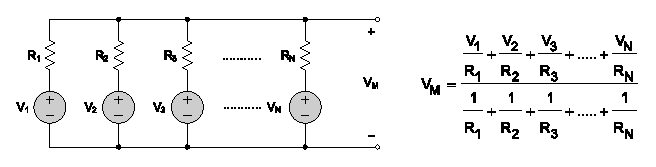
\includegraphics[width=0.70\textwidth]{resources/figura10.eps}
\end{figure}

Se calcula el voltaje de \emph{Thévenin} por medio del método de voltajes de
nodo:

\begin{equation*}
    \frac{V_{TH} - V_1}{R_1} + \frac{V_{TH} - V_2}{R_2} +
    \frac{V_{TH} - V_3}{R_3} + \cdots + \frac{V_{TH} - V_N}{R_N} = 0
\end{equation*}
\begin{equation*}
    \frac{V_{TH}}{R_1} - \frac{V_1}{R_1} +
    \frac{V_{TH}}{R_2} - \frac{V_2}{R_2} +
    \frac{V_{TH}}{R_3} - \frac{V_3}{R_3} + \cdots +
    \frac{V_{TH}}{R_N} - \frac{V_N}{R_N} = 0
\end{equation*}
\begin{equation*}
    \frac{V_{TH}}{R_1} + \frac{V_{TH}}{R_2} +
    \frac{V_{TH}}{R_3} + \cdots + \frac{V_{TH}}{R_N} =
    \frac{V_1}{R_1} + \frac{V_2}{R_2} +
    \frac{V_3}{R_3} + \cdots + \frac{V_N}{R_N} 
\end{equation*}
\begin{equation*}
    V_{TH}\left(\frac{1}{R_1} + \frac{1}{R_2} +
    \frac{1}{R_3} + \cdots + \frac{1}{R_N}\right) =
    \frac{V_1}{R_1} + \frac{V_2}{R_2} +
    \frac{V_3}{R_3} + \cdots + \frac{V_N}{R_N} 
\end{equation*}
\begin{equation*}
    V_{TH}= \dfrac{\dfrac{V_1}{R_1} + \dfrac{V_2}{R_2} +
    \dfrac{V_3}{R_3} + \cdots + \dfrac{V_N}{R_N}}{\dfrac{1}{R_1} +
    \dfrac{1}{R_2} + \dfrac{1}{R_3} + \cdots + \dfrac{1}{R_N}}
\end{equation*}

\end{enumerate}

\section{Conclusiones}
Se demostró experimentalmente el teorema de \emph{Thévenin}, mediante la
medición de circuitos tanto en laboratorio, como mediante una simulación.

Adicionalmente se analizó el puente de \emph{Wheatstone} y sus condiciones de
equilibrio, útil para la medición de resistencias.

\end{document}

